%-----------------------------------------------------------------------------%
%	Packages & Other Configurations
%-----------------------------------------------------------------------------%
\RequirePackage{fix-cm}  % Fix Font shape `OT1/cmr/m/n' size substitution.
\documentclass[a4paper,10pt]{article}
\usepackage[top=0.3in, bottom=0.3in, left=1in, right=0.9in]{geometry}
\usepackage[utf8]{inputenc} %add acents
\usepackage{setspace} % command \doublespacing etc...
%\usepackage{lineno} % number lines
\usepackage{epsf,epsfig} % includegraphics [pdf, png etc]
\usepackage{amsmath} %adicionei esse pacote pra vc poder usar o draft%
\usepackage{textcomp} %símbolos de texto
\usepackage{natbib} % bibtex - adicionar referencia
% \usepackage{url} % for bibtex - configuracoes de urls
\usepackage{tabularx} % for tables
\usepackage[hidelinks]{hyperref}  % Add URL links.
% \usepackage[bookmarks=false,colorlinks=true,urlcolor={green},linkcolor={green},pdfstartview={XYZ null null 1.22}]{hyperref} %all references
\usepackage{tikz}
\usepackage{lscape}
\usepackage{siunitx}
\usepackage{geometry}

%-----------------------------------------------------------------------------%
%	Adicionar a Watermark
%-----------------------------------------------------------------------------%
\usepackage{draftwatermark}
\SetWatermarkAngle{45}
\SetWatermarkLightness{0.9}
\SetWatermarkFontSize{5cm}
\SetWatermarkScale{0.3}
\SetWatermarkText{Prática 2 - Oceanografia}
%-----------------------------------------------------------------------------%
%	Informações sobre o PDF
%-----------------------------------------------------------------------------%
\pdfinfo{%
  /Title    (GEO232 - Prática 2)
  /Author   (Ju Leonel)
  /Creator  (Ju Leonel)
  /Producer (Ju Leonel)
  /Subject  (Intro oceanografias)
  /Keywords (Intro oceanografia, prática 2)}

%-----------------------------------------------------------------------------%
%	Documento
%-----------------------------------------------------------------------------%
\title{GEO232 - Introdução à Oceanografia - IGEO-UFBA}
\author{\vspace{-10ex}}
\date{\vspace{-10ex}}

\geometry{hmargin=1cm,vmargin=1cm}

\begin{document}
\phantom{}

\vspace{2cm}

{\small
\begin{center}
  \begin{tabular}{l l r r}
    \multicolumn{4}{l}{\Large{{\bf Descrição do Testemunho}}} \\
    \hline
                        &                  & \multicolumn{1}{l}{{\bf Percentagem de}}          & \multicolumn{1}{l}{{\bf Profundidade da}}    \\
                        &                  & \multicolumn{1}{l}{{\bf carbonato de cálcio nos}} & \multicolumn{1}{l}{{\bf coluna d'água}}    \\
    {\bf Identificação} & {\bf Descrição}  & \multicolumn{1}{l}{{\bf primeiros 10 cm}}         & \multicolumn{1}{l}{{\bf (metros)}} \\
    \hline
    \multicolumn{4}{l}{\phantom{}} \\
    \multicolumn{4}{l}{{\bf Oceano A}} \\
    1 & Fragmentos de rochas vulcânicas, algumas vasas                  & -- & 1500 \\
    2 & 10 m de vasas carbonáticas, alguns fragmentos vulcânicos        & 90 & 2000 \\
      & e cinzas vulcânicas no topo                                     &    &      \\
    3 & 10 m de vasas, nódulos de Mn no topo                            & 80 & 3000 \\
    4 & 9 m de vasas, nódulos de Mn no topo                             & 75 & 4000 \\
    5 & 3 m de argila vermelha sobre 3 m de vasas carbonáticas          & 15 & 5000 \\
    6 & 8 m de argila vermelha                                          &  3 & 6000 \\
    7 & 9 m de argila vermelha                                          &  5 & 7000 \\
    8 & 1 m de areia fina no topo e areia grossa na base,               & 15 & 4500 \\
      & sobre 50 cm de lama, sobre 60 cm                     &    &      \\
      & de areia, sobre 3 m de argila vermelha                          &    &      \\
    9 & 6 m de camadas alternadas de argila vermelha e silte com      & -- & 1000 \\
      & algumas camadas de areia fina a grossa, uma camada de areia     &    &      \\
      & na base e cascalho no fundo                                     &    &      \\
    \multicolumn{4}{l}{\phantom{}} \\
    \multicolumn{4}{l}{{\bf Oceano B}} \\
    10 & 4 m de areia grossa e cascalho                                 & -- &  500 \\
    11 & 7 m de silte com camadas de areia e cascalho de                & -- & 1500 \\
       & aproximadamente 40 cm de espessura                             &    &      \\
    12 & 9 m de lama com areia fina e camadas de silte                  & -- & 3000 \\
       & de aproximadamente 20 cm de espessura                          &    &      \\
    13 & 10 m de argilas e lama, diversas camadas de areia e            &  6 & 4000 \\
       & silte de aproximadamente 10 cm de espessura                    &    &      \\
    14 & 10 m de lama com poucas camadas de silte com                   & 62 & 3000 \\
       & aproximadamente 5 cm de espessura                              &    &      \\
    15 & 10 m de vasas                                                  & 78 & 2000 \\
    16 & Fragmentos de rochas (basalto) e cinzas vulcânicas             & -- & 1500 \\
    \hline
  \end{tabular}
\end{center}
}

\newpage


\def\width{9}
\def\hauteur{8}


\phantom{}

\vspace{2cm}

\begin{center}
  \begin{itemize}
    \item[1. (a)] Plote os dados de carbonato de cálcio versus a profundidade para os testemunhos  1--16. Use círculos abertos para o Oceano A e círculos fechados para o Oceano B (não é necessário ligar os pontos). Se não houver valor de CaCO$_3$, não plote. 
    
     \item[1. (b)] Sugira motivos pelo quais há uma drásticas mudanças nos valores de CaCO$_3$ a partir da profundidade de 4000 m. 
     
  \end{itemize}
\end{center}

\vspace{2cm}

\begin{center}
  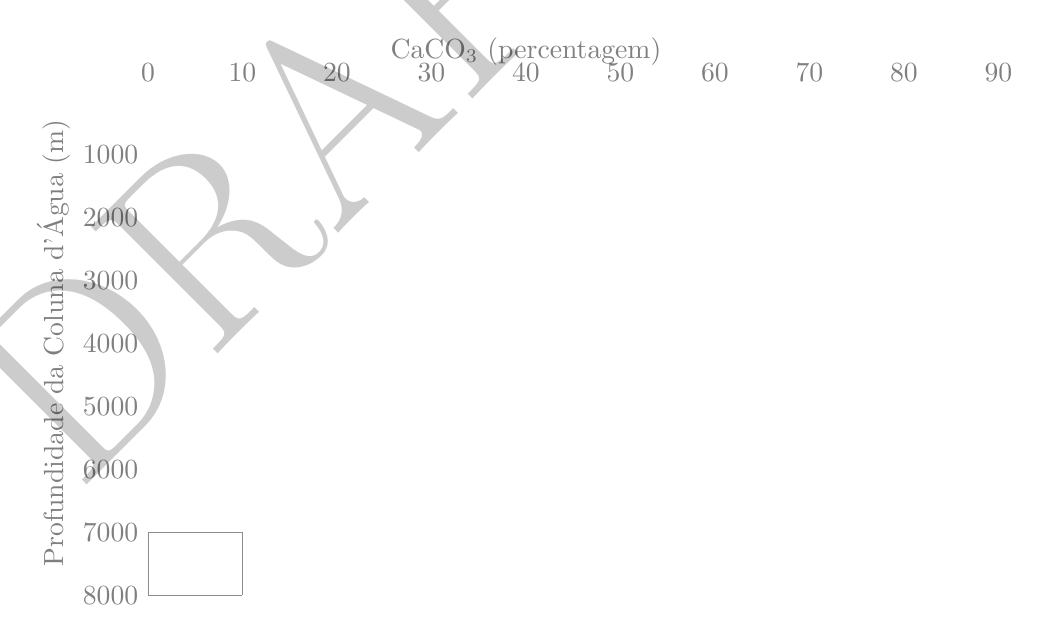
\begin{tikzpicture}[x=12mm, y=8mm, semitransparent]
  % Grid.
  \draw[xstep=12mm, ystep=8mm, line width=0.1mm, black!90!white] (0,0) grid (\width,\hauteur);
  % y-tickslabels.
  \draw[black] (4, 9) node[anchor=north] {CaCO$_3$ (percentagem)};
  % x-tickslabels.
  \draw[black] ( 0, 8) node[anchor=south] {0};
  \draw[black] ( 1, 8) node[anchor=south] {10};
  \draw[black] ( 2, 8) node[anchor=south] {20};
  \draw[black] ( 3, 8) node[anchor=south] {30};
  \draw[black] ( 4, 8) node[anchor=south] {40};
  \draw[black] ( 5, 8) node[anchor=south] {50};
  \draw[black] ( 6, 8) node[anchor=south] {60};
  \draw[black] ( 7, 8) node[anchor=south] {70};
  \draw[black] ( 8, 8) node[anchor=south] {80};
  \draw[black] ( 9, 8) node[anchor=south] {90};
  % y-tickslabels.
  \draw[black] (-1, 4) node[rotate=90] {Profundidade da Coluna d'Água (m)};
  % y-tickslabels.
  \draw[black] ( 0, 7) node[anchor=east] {1000};
  \draw[black] ( 0, 6) node[anchor=east] {2000};
  \draw[black] ( 0, 5) node[anchor=east] {3000};
  \draw[black] ( 0, 4) node[anchor=east] {4000};
  \draw[black] ( 0, 3) node[anchor=east] {5000};
  \draw[black] ( 0, 2) node[anchor=east] {6000};
  \draw[black] ( 0, 1) node[anchor=east] {7000};
  \draw[black] ( 0, 0) node[anchor=east] {8000};
  \end{tikzpicture}
\end{center}

\newpage

\def\width{17}
\def\hauteur{8}


\phantom{}

\vspace{2cm}

\begin{center}
  \begin{itemize}
    \item[2.(a)] No gráfico abaixo, plote o perfil de profundidade de cada um dos testemunhos dos oceanos A e B. No perfil, use canetas de diferentes cores para indicar o tipo de sedimento predominante em cada um dos testemunhos. Por exemplo, use vermelho para argilas vermelhas, azul para vasas, amarelo para areias, siltes e lamas terrígenas, e preto para rochas vulcânicas e basalto. 
  
   \item[2.(b)] Faça uma comparação entre os dois oceanos (A e B) sugerindo motivos para as diferençãs na distribuição dos sedimentos. 
   
  \end{itemize}
\end{center}

\vspace{2cm}

\begin{center}
  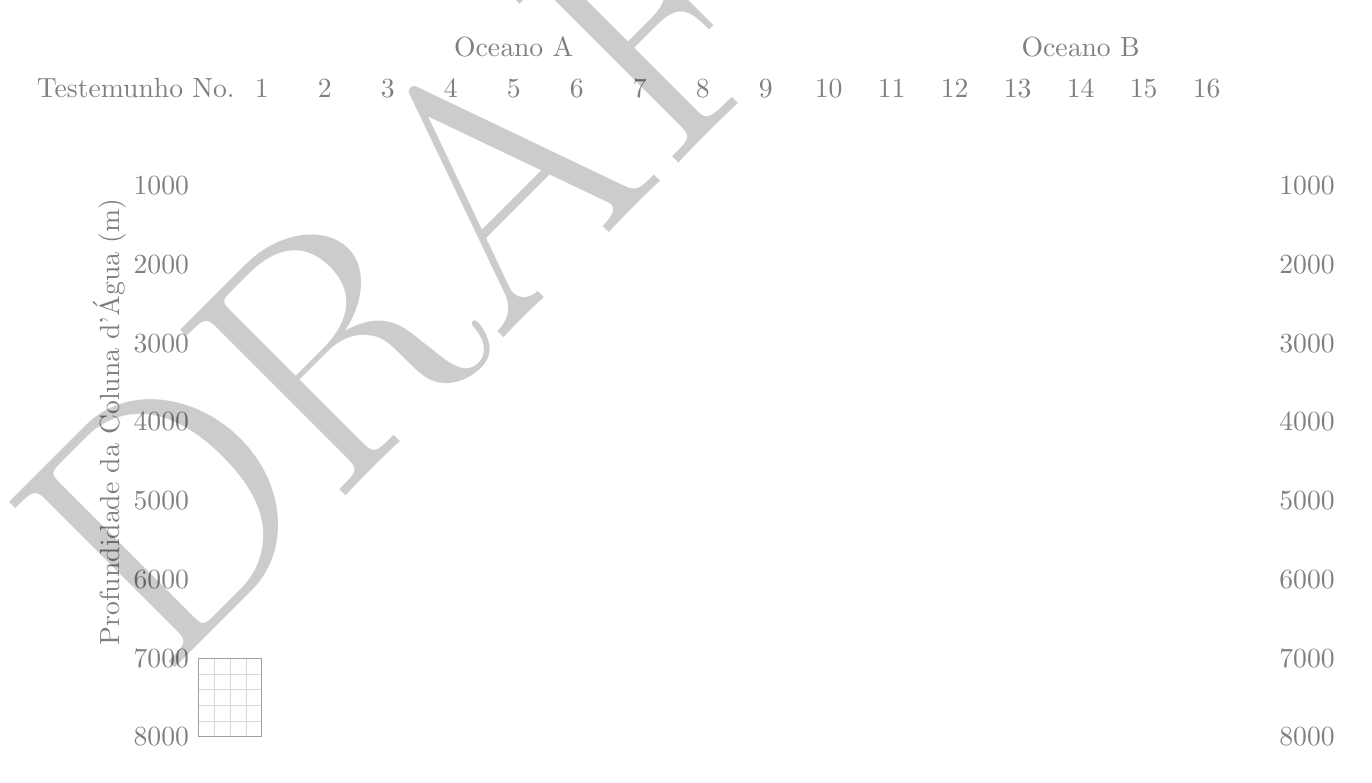
\begin{tikzpicture}[x=8mm, y=10mm, semitransparent]
  % Grid.
  \draw[xstep=8mm, ystep=10mm, line width=0.1mm, black!90!white] (0,0) grid (\width,\hauteur);
  \draw[step=2mm, line width=0.1mm, black!30!white] (0,0) grid (\width,\hauteur);
  % x-tickslabels.
  \draw[black] ( 1, 8) node[anchor=south] {1};
  \draw[black] ( 2, 8) node[anchor=south] {2};
  \draw[black] ( 3, 8) node[anchor=south] {3};
  \draw[black] ( 4, 8) node[anchor=south] {4};
  \draw[black] ( 5, 8) node[anchor=south] {5};
  \draw[black] ( 6, 8) node[anchor=south] {6};
  \draw[black] ( 7, 8) node[anchor=south] {7};
  \draw[black] ( 8, 8) node[anchor=south] {8};
  \draw[black] ( 9, 8) node[anchor=south] {9};
  \draw[black] (10, 8) node[anchor=south] {10};
  \draw[black] (11, 8) node[anchor=south] {11};
  \draw[black] (12, 8) node[anchor=south] {12};
  \draw[black] (13, 8) node[anchor=south] {13};
  \draw[black] (14, 8) node[anchor=south] {14};
  \draw[black] (15, 8) node[anchor=south] {15};
  \draw[black] (16, 8) node[anchor=south] {16};
  % x-labels.
  \draw[black] (-1, 8) node[anchor=south] {Testemunho No.};
  \draw[black] (5, 9) node[anchor=north] {Oceano A};
  \draw[black] (14, 9) node[anchor=north] {Oceano B};
  % y-labels.
  \draw[black] (-1, 4) node[anchor=south, rotate=90] {Profundidade da Coluna d'Água (m)};
  % y-tickslabels left.
  \draw[black] (0, 7) node[anchor=east] {1000};
  \draw[black] (0, 6) node[anchor=east] {2000};
  \draw[black] (0, 5) node[anchor=east] {3000};
  \draw[black] (0, 4) node[anchor=east] {4000};
  \draw[black] (0, 3) node[anchor=east] {5000};
  \draw[black] (0, 2) node[anchor=east] {6000};
  \draw[black] (0, 1) node[anchor=east] {7000};
  \draw[black] (0, 0) node[anchor=east] {8000};
  % y-tickslabels right.
  \draw[black] (17, 7) node[anchor=west] {1000};
  \draw[black] (17, 6) node[anchor=west] {2000};
  \draw[black] (17, 5) node[anchor=west] {3000};
  \draw[black] (17, 4) node[anchor=west] {4000};
  \draw[black] (17, 3) node[anchor=west] {5000};
  \draw[black] (17, 2) node[anchor=west] {6000};
  \draw[black] (17, 1) node[anchor=west] {7000};
  \draw[black] (17, 0) node[anchor=west] {8000};
  \end{tikzpicture}
\end{center}


\end{document}
